\chapter{Simulação do Sistema} \label{secao:simulacao_sistema}

A simulação foi realizada no ambiente Simulink em conjunto com o Simscape, de forma a facilitar a implementação de circuitos elétricos.

Para simular o sistema é necessário ter como entrada uma curva de irradiância. A curva aqui utilizada é baseada em um modelo de órbita desenvolvido no LCS/UFSC \cite{slongo2016}, o qual considera uma órbita equatorial, que apresenta regiões de eclipse, nas quais a Terra fica entre o satélite e o Sol (pior caso em termos de entrada de energia). A curva é apresentada na Figura \ref{figura_irradiancia_simulacao}.

\begin{figure}[!htpb]
\begin{center}
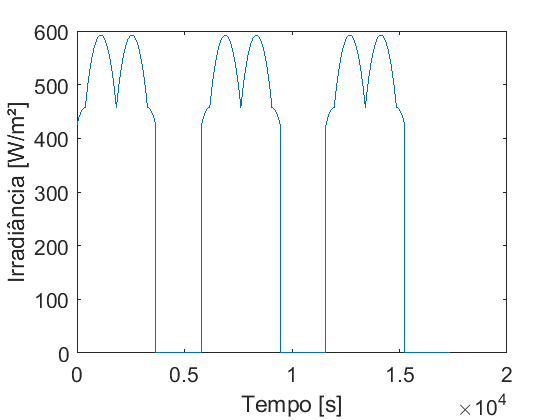
\includegraphics[scale=0.5]{figures/simulatedIrradiance.png}
\caption{Irradiância}
\label{figura_irradiancia_simulacao}
\end{center}
\end{figure}

O modelo do painel solar apresentado no capítulo \ref{secao:painel solar} foi implementado utilizando a linguagem Simscape, dentro do ambiente Simulink. Devido ao fato de que, pela geometria do \textit{cubesat}, apenas três faces recebem iluminação ao mesmo tempo, foram considerados três painéis conectados ao sistema.

O conversor \textit{Boost} foi simulado de forma bastante simples através de uma fonte de tensão controlada, de forma que a amplitude da fonte representa o ganho de tensão do conversor. O controle da amplitude foi realizado pelo algoritmo \gls{peo} implementado através do bloco \textit{MATLAB Function}.

A potência consumida pelas cargas foi simulada através de uma fonte de corrente controlada pelo modelo do capítulo \ref{secao:modelagem_cargas} e alimentada por um conversor DC-DC ideal.

Por fim as baterias foram simuladas utilizando o bloco \textit{Generic Battery} do Simscape.

Pode-se visualizar a atuação do algoritmo \gls{peo} na Figura \ref{figura_simulacao_tensao_painel_solar}, sendo que nos momentos onde existe luz no painel solar a tensão é variada de forma a manter o painel operando no \gls{mpp}.

\begin{figure}[!htpb]
\begin{center}
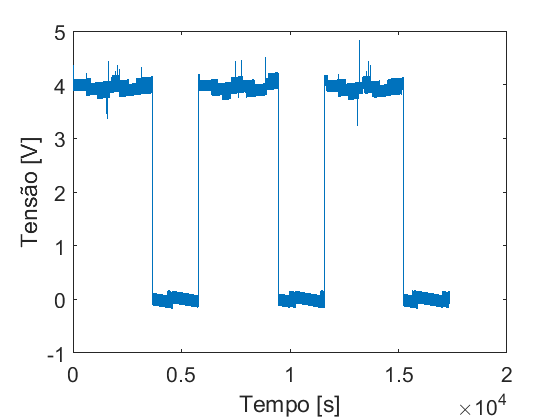
\includegraphics[scale=0.5]{figures/simulatedSolarPanelVoltage.png}
\caption{Tensão do Painel Solar}
\label{figura_simulacao_tensao_painel_solar}
\end{center}
\end{figure}

A corrente fornecida pelos painéis está na Figura \ref{figura_simulacao_corrente_painel_solar}. Pode-se ver que, assim como a potência entregue (Figura \ref{figura_simulacao_potencia_painel_solar}), ela acompanha a curva de irradiância, porém a tensão não, o que mostra o funcionamento do \gls{mppt}. 

\begin{figure}[!htpb]
\begin{center}
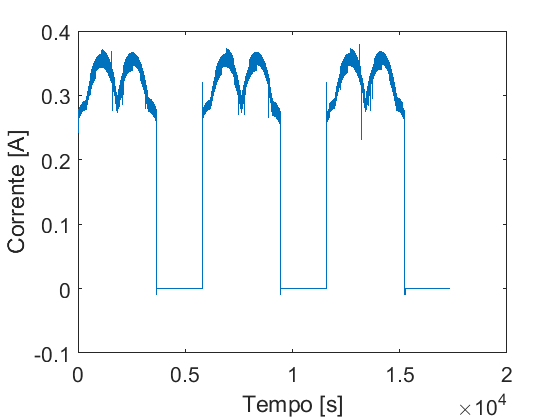
\includegraphics[scale=0.5]{figures/simulatedSolarPanelCurrent.png}
\caption{Corrente do Painel Solar}
\label{figura_simulacao_corrente_painel_solar}
\end{center}
\end{figure}

\begin{figure}[!htpb]
\begin{center}
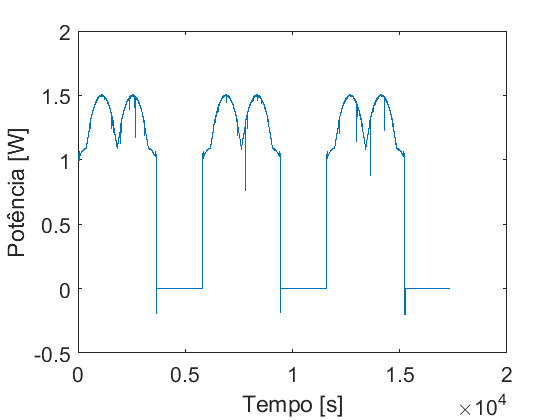
\includegraphics[scale=0.5]{figures/simulatedSolarPanelPower.png}
\caption{Potência do Painel Solar}
\label{figura_simulacao_potencia_painel_solar}
\end{center}
\end{figure}

As tensões das baterias podem ser vistas nas figuras \ref{figura_simulacao_tensao_bat1} e \ref{figura_simulacao_tensao_bat2}. Como podemos ver pela pequena diminuição na tensão, as cargas estão praticamente equilibradas com a entrada de energia.

\begin{figure}[!htpb]
\begin{center}
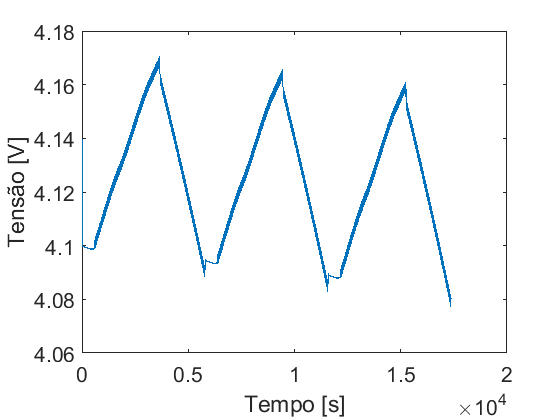
\includegraphics[scale=0.5]{figures/simulatedBatteryVoltage1.png}
\caption{Tensão da Bateria 1}
\label{figura_simulacao_tensao_bat1}
\end{center}
\end{figure}

\begin{figure}[!htpb]
\begin{center}
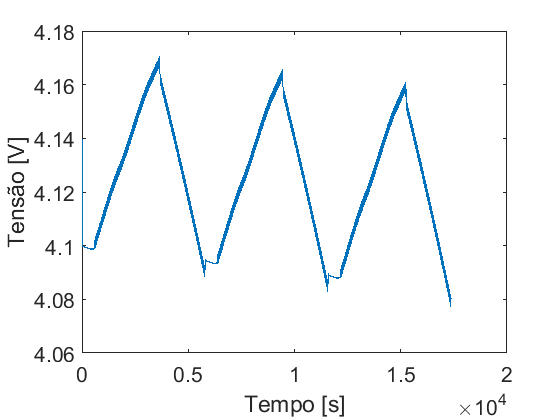
\includegraphics[scale=0.5]{figures/simulatedBatteryVoltage2.png}
\caption{Tensão da Bateria 2}
\label{figura_simulacao_tensao_bat2}
\end{center}
\end{figure}